\documentclass{internoise2012}

\usepackage{lipsum}
\usepackage{booktabs}
\usepackage{url}

\begin{document}

\title{A \LaTeX{} class for preparing 2012 Inter-Noise papers}

\author{Cameron Fackler\thanks{email: facklc@rpi.edu}}
\affil{Graduate Program in Architectural Acoustics, School of
  Architecture,\\Rensselaer Polytechnic Institute, Troy, New York, USA
  12180}

\author{Second Author\thanks{email: someone@somewhere.com}}
\author{Third Author\thanks{email: someoneelse@somewhere.com}}
\affil{Another Place, Another School,\\Anytown, USA}

\maketitle

\begin{abstract}
  This is a \LaTeX{} \texttt{documentclass} for preparing conference
  papers adhering to the specifications for the 2012 InterNoise
  proceedings. This sample document demonstrates proper useage of the
  class. The original paper formatting specifications can be
  downloaded from
  \url{http://internoise2012.com/callabstracts.shtml}. Refer to the
  source of this document, \texttt{InterNoise2012Sample.tex}, for a
  working example of class usage.
\end{abstract}

\section{Introduction}

Documents prepared using this class should follow standard \LaTeX{}
markup. As per the conference guidelines, only Section and Subsection
headings are numbered. Section names defined using the
\texttt{\textbackslash{}section\{\}} command will be capitalized
automatically. For subsections defined with
\texttt{\textbackslash{}subsection\{\}}, the user is responsible for
following the official guidelines and capitalizing only the first word.

\section{Front matter}

The front matter generally follows standard \LaTeX{} practice, with
some convenience differences for entering authors and
affiliations. The title is specified using the normal
\texttt{\textbackslash{}title\{\}} command. No date should be entered.

To ease the inputting of multiple author and affiliation groups, this
class uses the functionality of the \texttt{authblk} package. All
authors should be entered invidually, with the
\texttt{\textbackslash{}author\{\}} command. Inside this command,
authors' email addresses are specified with the
\texttt{\textbackslash{}thanks\{\}} command. For example, the author
of the document class entered himself as
\begin{verbatim}
\author{Cameron Fackler\thanks{email: facklc@rpi.edu}}
\end{verbatim}

Affiliations are entered using the \texttt{\textbackslash{}affil\{\}}
command, immediately following the \texttt{author} command. If
multiple authors share a common affiliation, each \texttt{author}
should be entered, followed by a single \texttt{affil}. Refer to the
source of this document for an example.

Once the paper title and all authors and affiliations have been
entered, the \texttt{\textbackslash{}maketitle} command is issued,
causing the conference logo, paper title, and author and affiliation
information to be output. The abstract is then entered using the
standard \texttt{abstract} environment.

\section{Body}

\subsection{Main Content}

Section titles should be entered with the \texttt{section}
command. They will be typeset in all capitals automatically. For
subsections, use the \texttt{subsection} command. To follow the
official paper guidelines, subsection names should have all major
words capitalized individually. The author is responsible to follow
this formatting: subsection titles are typeset as entered.

\subsection{Tables and Figures}

Tables and figures may be input throughout the document using the
standard \LaTeX floating environments. This document class will gather
them at the end of the document automatically.

Note that table captions should appear above tables, while figure
captions should appear below their respective figure. The author must
ensure that commands within the \texttt{table} and \texttt{figure}
environments are entered in the correct order. Namely, in a
\texttt{table} environment, the caption should be entered above the
\texttt{tabular} command. In a \texttt{figure} environment, the
caption should be entered following any \texttt{includegraphics} or
other figure content commands. Refer to the source of this document
for examples.

For nicer looking tables, it is recommended that the paper author
utilize the \texttt{booktabs} \LaTeX package. The example table in the
source of this paper demonstrates the slight syntax differences
required for this package.

\begin{table}[ht]
  \centering
  \caption{Example table. Borrowed and slightly modified from the
    official paper guidelines.}
  \begin{tabular}{lccc}
    % instead of \hline\hline use \toprule for booktabs
    \toprule
    Layer & 1 & 2 & 3 \\
    % lines in the table body are created with \midrule
    \midrule
    Material & anechoic & decoupling & steel \\
    Thickness (m) & 0.04 & 0.01 & 0.01 \\
    Loss Factor & 0.2 & 0.1 & 0.01 \\
    % again replace \hline\hline
    \bottomrule
  \end{tabular}
  \label{tab:example-table}
\end{table}

\begin{figure}[ht]
  \centering
  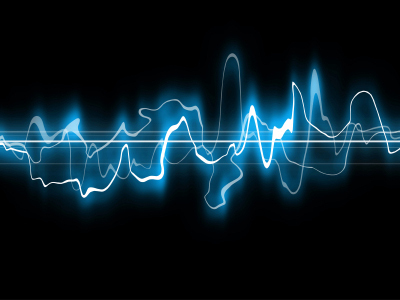
\includegraphics[width=3in]{sound}
  \caption{Example figure. This figure has a long caption, which
    should demonstrate how it wraps around if necessary. Just to be
    certain, let's put one more sentence in the figure caption. And
    one more, just to be extra sure for good measure.}
  \label{fig:example-figure}
\end{figure}

\subsection{References}

This document class utilizes functionality of the \texttt{natbib}
package to simplify reference management. Multiple simultaneous
citations should be combined into one \texttt{cite} command, as in
\texttt{\textbackslash{}cite\{allard2009,beranek2006,biot1956\}}.\cite{allard2009,beranek2006,biot1956}
This will cause the citations to be compressed if possible, such that
a range is specified.

Ensure that the file \texttt{jasanum.bst} remains in the same folder
as the \LaTeX source. It is used internally by the document class to
format references as they appear in JASA.

\subsection{Equations}

Equations are entered using the standard \texttt{equation}
environment, such as
\begin{equation}
  \frac{1}{2} e^{i \pi} - 4\gamma^3,
\end{equation}
where $\pi$ and $\gamma$ are dummy variables.

\bibliography{sample}

\end{document}
